% -*- program:xelatex -*-

\documentclass[t]{beamer}\usepackage[]{graphicx}\usepackage[]{color}
%% maxwidth is the original width if it is less than linewidth
%% otherwise use linewidth (to make sure the graphics do not exceed the margin)
\makeatletter
\def\maxwidth{ %
  \ifdim\Gin@nat@width>\linewidth
    \linewidth
  \else
    \Gin@nat@width
  \fi
}
\makeatother

\definecolor{fgcolor}{rgb}{0.345, 0.345, 0.345}
\newcommand{\hlnum}[1]{\textcolor[rgb]{0.686,0.059,0.569}{#1}}%
\newcommand{\hlstr}[1]{\textcolor[rgb]{0.192,0.494,0.8}{#1}}%
\newcommand{\hlcom}[1]{\textcolor[rgb]{0.678,0.584,0.686}{\textit{#1}}}%
\newcommand{\hlopt}[1]{\textcolor[rgb]{0,0,0}{#1}}%
\newcommand{\hlstd}[1]{\textcolor[rgb]{0.345,0.345,0.345}{#1}}%
\newcommand{\hlkwa}[1]{\textcolor[rgb]{0.161,0.373,0.58}{\textbf{#1}}}%
\newcommand{\hlkwb}[1]{\textcolor[rgb]{0.69,0.353,0.396}{#1}}%
\newcommand{\hlkwc}[1]{\textcolor[rgb]{0.333,0.667,0.333}{#1}}%
\newcommand{\hlkwd}[1]{\textcolor[rgb]{0.737,0.353,0.396}{\textbf{#1}}}%

\usepackage{framed}
\makeatletter
\newenvironment{kframe}{%
 \def\at@end@of@kframe{}%
 \ifinner\ifhmode%
  \def\at@end@of@kframe{\end{minipage}}%
  \begin{minipage}{\columnwidth}%
 \fi\fi%
 \def\FrameCommand##1{\hskip\@totalleftmargin \hskip-\fboxsep
 \colorbox{shadecolor}{##1}\hskip-\fboxsep
     % There is no \\@totalrightmargin, so:
     \hskip-\linewidth \hskip-\@totalleftmargin \hskip\columnwidth}%
 \MakeFramed {\advance\hsize-\width
   \@totalleftmargin\z@ \linewidth\hsize
   \@setminipage}}%
 {\par\unskip\endMakeFramed%
 \at@end@of@kframe}
\makeatother

\definecolor{shadecolor}{rgb}{.97, .97, .97}
\definecolor{messagecolor}{rgb}{0, 0, 0}
\definecolor{warningcolor}{rgb}{1, 0, 1}
\definecolor{errorcolor}{rgb}{1, 0, 0}
\newenvironment{knitrout}{}{} % an empty environment to be redefined in TeX

\usepackage{alltt}

\usepackage{geometry}
\usepackage{graphicx}
\usepackage{amssymb}
\usepackage{epstopdf}
\usepackage{amsmath}    % this permits text in eqnarray among other benefits
\usepackage{color}            % gives color options
\usepackage{url}    % produces hyperlinks
\usepackage[english]{babel}
%\usepackage[latin1]{inputenc}
\usepackage{colortbl} % allows for color usage in tables
\usepackage{multirow} % allows for rows that span multiple rows in tables
\usepackage{xcolor}   % this package has a variety of color options
\usepackage{calc}
\usepackage{multicol}
%\usepackage{minted}
\usepackage{wrapfig}
\usepackage{textcomp}


\usetheme{metropolis} 

\setbeamertemplate{navigation symbols}{}

%User defined colors: See colors section
\xdefinecolor{oiBlue}{rgb}{0.15, 0.35, 0.55}
\xdefinecolor{gray}{rgb}{0.5, 0.5, 0.5}
\xdefinecolor{darkGray}{rgb}{0.3, 0.3, 0.3}
\xdefinecolor{darkerGray}{rgb}{0.2, 0.2, 0.2}
\xdefinecolor{rubineRed}{rgb}{0.89,0,0.30}
\xdefinecolor{linkCol}{rgb}{0.11,0.49,0.95}	
\xdefinecolor{irishGreen}{rgb}{0,0.60,0}	
\xdefinecolor{darkturquoise}{rgb}{0.44, 0.58, 0.86}
\definecolor{lightGreen}{rgb}{0.533,0.765,0.42}

\setbeamercolor*{palette primary}{fg=white,bg= oiBlue!70}
\setbeamercolor*{palette secondary}{fg=black,bg= oiBlue!20!white}
\setbeamercolor*{palette tertiary}{fg=white,bg= oiBlue!80!black!90}
\setbeamercolor*{palette quaternary}{fg=white,bg= oiBlue}

\setbeamercolor{structure}{fg= oiBlue}
\setbeamercolor{frametitle}{bg= oiBlue!70}

\setbeamercolor{disc body}{bg=oiBlue!20!white!80,fg=oiBlue!80!black!90}
\setbeamercolor{disc title}{bg=oiBlue!40!white!60,fg=oiBlue!70!black!100}


\setbeamertemplate{blocks}[shadow=false]


\newcommand{\removepagenumbers}{% 
  \setbeamertemplate{footline}{
    %
    \begin{beamercolorbox}[colsep=1.5pt]{upper separation line foot}
    \end{beamercolorbox}
    \begin{beamercolorbox}[ht=2.5ex,dp=1.125ex,%
      leftskip=.3cm,rightskip=.3cm plus1fil]{author in head/foot}%
      \leavevmode{\usebeamerfont{author in head/foot}\insertshortauthor}%
%      \hfill%
%      {\usebeamerfont{author in head/foot}\usebeamercolor[fg]{institute in head/foot}\insertshortinstitute}%
    \end{beamercolorbox}%
    \begin{beamercolorbox}[ht=2.5ex,dp=1.125ex,%
      leftskip=.3cm,rightskip=.3cm plus1fil]{title in head/foot}%
      {\usebeamerfont{title in head/foot}\insertshorttitle}%
      \hfill%
      {\usebeamerfont{author in head/foot}\usebeamercolor[fg]{institute in head/foot}\insertshortinstitute}%
    \end{beamercolorbox}%
    \begin{beamercolorbox}[colsep=1.5pt]{lower separation line foot}
    \end{beamercolorbox}
    }
} 

\newenvironment{twocol}[4]{
\begin{columns}[t]
\column{#1\textwidth}
#3
\column{#2\textwidth}
#4
\end{columns}
}

\newcommand{\disc}[2]{
\begin{beamerboxesrounded}[shadow = true, lower = disc body, upper = disc title]{#1}
#2
\end{beamerboxesrounded}
}


\AtBeginSection[] 
{ 
  \addtocounter{framenumber}{-1} 
  % 
  {\removepagenumbers 
    \begin{frame}<beamer> 
    \tableofcontents[currentsection] 
  \end{frame} 
  } 
} 

\usepackage{bm}
\usepackage{isotope}
\usepackage{appendixnumberbeamer}
\usepackage{dsfont}

\newcommand{\PM}{$\text{PM}_{2.5}$ }


\definecolor{redhl}{rgb}{0.98,0.29,0.28}
\definecolor{yellowhl}{rgb}{0.98,0.87,0.28}
\newcommand{\hlr}[1]{\fcolorbox{redhl}{white}{$\displaystyle #1$}}
\newcommand{\hly}[1]{\fcolorbox{yellowhl}{white}{$\displaystyle #1$}}

\newcommand{\vvfill}{\vskip0pt plus 1filll}

\title[GPU GPs]{GPUs and the computational efficiency\\ of Gaussian process based models}
\author{Colin Rundel}
\date{April 25, 2016}
\institute[Duke]{Duke University}
\IfFileExists{upquote.sty}{\usepackage{upquote}}{}
\begin{document}

\begin{frame}[plain]
\titlepage
\end{frame}



%==================================================================================================

\section{Background}
\addtocounter{framenumber}{-1} 

%==================================================================================================

\begin{frame}
\frametitle{What is a Gaussian Process}

A statistical distribution that describes observations that arise from a continuous domain (e.g. space, time), whereby any subset of points within that domain have a multivariate normal distribution.

\[\underset{n \times 1}{X} \sim \mathcal{N}(\underset{n \times 1}{\mu}, \underset{n \times n}{\Sigma})\]


\end{frame}


\begin{frame}
\frametitle{The problem with GPs ...}

Gaussian process models are difficult to scale to large problems:

\begin{align*}
&\text{Evaluate the (log) likelihood?}\\
%
&\qquad -\frac{1}{2} \log |\Sigma| - \frac{1}{2} (\bm{x}-\bm{\mu})' \bm{\Sigma}^{-1} (\bm{x}-\bm{\mu}) - \frac{n}{2}\log 2\pi
&\color{redhl}{\mathcal{O}\left(n^3\right)}\\
\\
&\text{Want a sample?}\\
%
&\qquad \bm{\mu} + \text{Chol}(\bm{\Sigma}) \times \bm{Z} \text{ with } Z_i \sim \mathcal{N}(0,1) 
&\color{redhl}{\mathcal{O}\left(n^3\right)} \\
\\
&\text{Update covariance parameter?} \\
%
&\qquad \{\Sigma\}_{ij} = \sigma^2 \exp(-\{d\}_{ij}\phi) 
&\color{yellowhl}{\mathcal{O}\left(n^2\right)}
\end{align*}
%


\end{frame}


%==================================================================================================

\begin{frame}[c]
\frametitle{A simple guide to computational complexity}

{\Large \begin{center}
\vfill
Linear complexity? \pause- Go for it \pause

\vspace{15mm}

Quadratic complexity? \pause- Pray \pause

\vspace{15mm}

Cubic complexity? \pause- Give up

\vfill
\end{center} }
\end{frame}

%==================================================================================================

\begin{frame}
\frametitle{Improving Cholesky}
    
\vspace{-8mm}

\begin{center}
\begin{knitrout}\footnotesize
\definecolor{shadecolor}{rgb}{0.969, 0.969, 0.969}\color{fgcolor}

{\centering 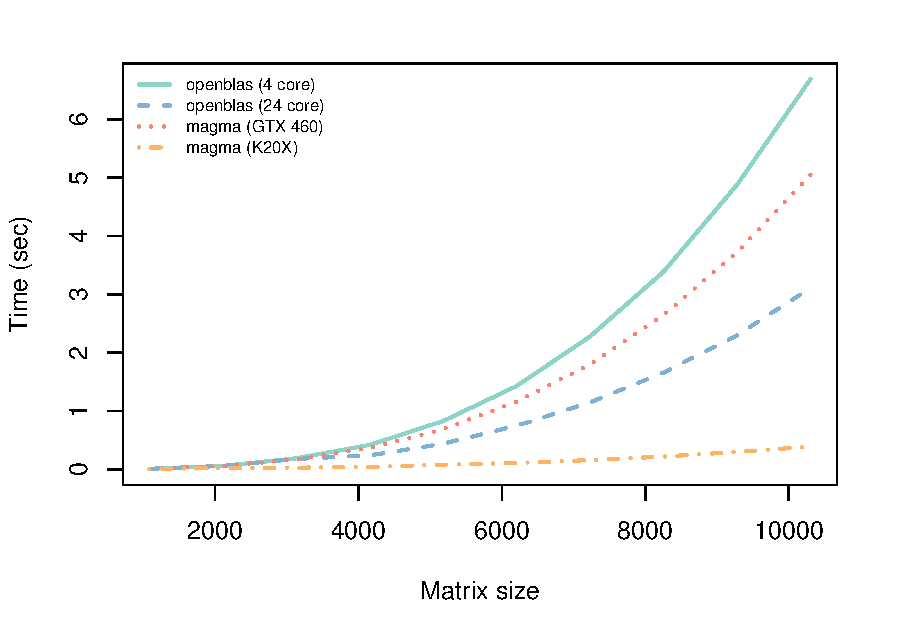
\includegraphics[width=\textwidth]{plots/unnamed-chunk-1-1} 

}



\end{knitrout}
\end{center}


\end{frame}

%==================================================================================================

\begin{frame}
\frametitle{Tools and Optimization}

\vfill

\begin{center}
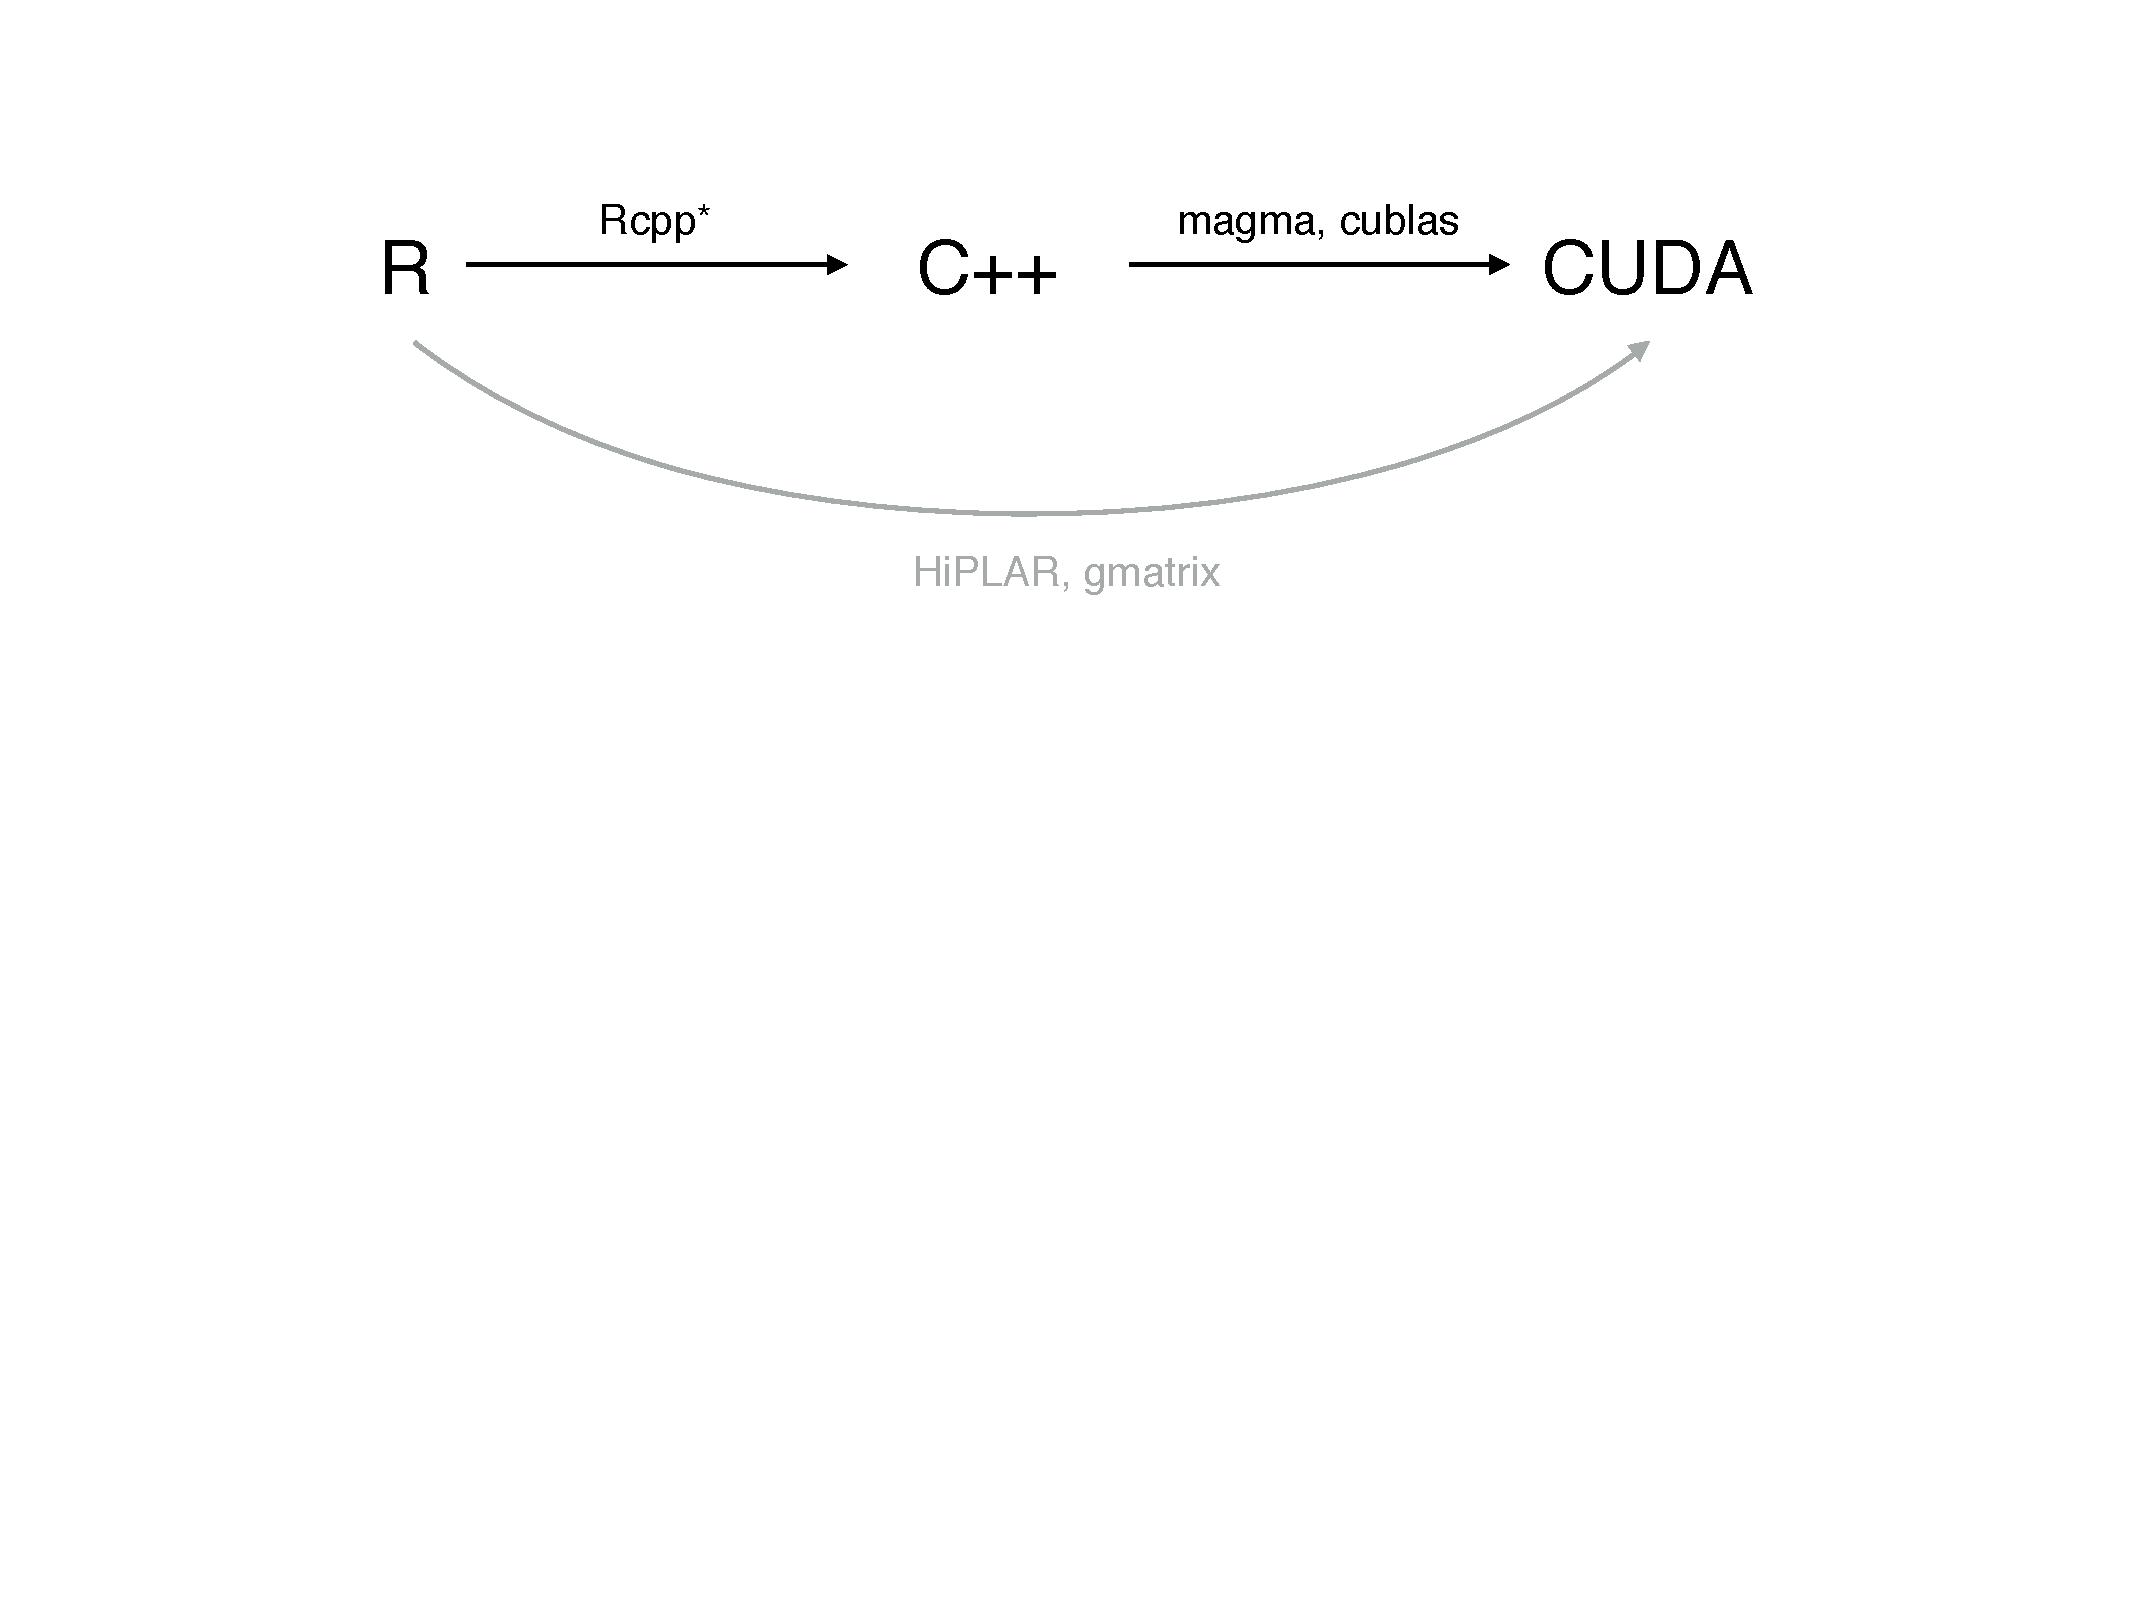
\includegraphics[width=0.9\textwidth]{figs/diagram.pdf}
\end{center}

\vfill

Regardless of tools or workflow, measuring / profiling performance is critical.

\vfill

\end{frame}

%==================================================================================================

\section{Migratory Bird Spatial Assignment Model}

%==================================================================================================

\begin{frame}
\frametitle{Background}

Using intrinsic markers (genetic and isotopic signals) for the purpose of inferring migratory connectivity.

\vspace{2mm}

\begin{itemize}
\item Existing methods are too coarse for most applications
\vspace{2mm}
\item Large amounts of data are available ( \textgreater{}150,000 feather samples from \textgreater{}500 species)
\vspace{2mm}
\item Genetic assignment methods are based on Wasser, et al. (2004)
\vspace{2mm}
\item Isotopic assignment methods are based on Wunder, et al. (2005)
\end{itemize}

\end{frame}

%==================================================================================================

\begin{frame}[t]
\frametitle{Data - DNA microsatellites and $\delta \isotope[2]{H}$}

\begin{columns}[t]
\column{0.5\textwidth}
Hermit Thrush \\
(\textit{Catharus guttatus}) \\
\vspace{2mm}
\begin{itemize}
\item 138 individuals
\item 14 locations
\item 6 loci
\item 9-27 alleles / locus
\end{itemize}
\column{0.5\textwidth}
Wilson's Warbler \\
(\textit{Wilsonia pusilla}) \\
\vspace{2mm}
\begin{itemize}
\item 163 individuals
\item 8 locations
\item 9 loci
\item 15-31 alleles / locus
\end{itemize}

\end{columns}

~\\

\begin{columns}[t]
\column{0.5\textwidth}
\begin{center}
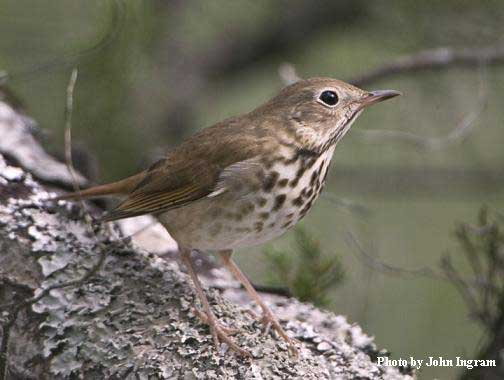
\includegraphics[width=0.65\textwidth]{figs/hermit_thrush.jpeg}
\end{center}
\column{0.5\textwidth}
\begin{center}
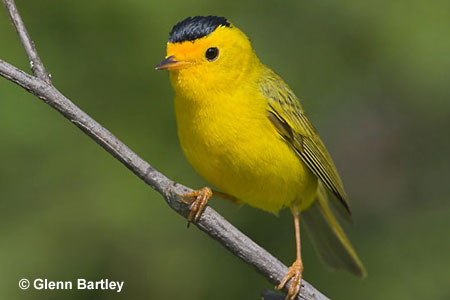
\includegraphics[width=0.65\textwidth]{figs/wilsons_warbler.jpeg}
\end{center}
\end{columns}


\end{frame}

%==================================================================================================

\begin{frame}
\frametitle{Allele Frequency Model}

For the allele $i$, from locus $l$, at location $k$

\begin{align*}
\bm{y}_{\cdot l k}|\bm{\Theta} &\sim \text{Mult}\left(\textstyle\sum_i y_{ilk},\: \bm{f}_{\cdot l k}\right) \\
\\
f_{ilk} &= \frac{\exp(\Theta_{ilk})}{\sum_i \exp(\Theta_{ilk})} \\
\\
\bm{\Theta}_{il}|\bm{\alpha},\bm{\mu} &\sim \mathcal{N}( \bm{\mu}_{il},\, \bm{\Sigma_{}}) \\
\end{align*}

\[ \left\{\Sigma\right\}_{ij} = \alpha_0 \, \exp \Big(-(\{d\}_{ij}/\alpha_1)^{\alpha_2} \Big) + \alpha_3 \, \mathds{1}_{i=j} \]

\end{frame}


%==================================================================================================


\begin{frame}
\frametitle{Genetic Assignment  Model}

Assignment model using Hardy-Weinberg equilibrium allowing for genotyping ($\delta$) and single amplification ($\gamma$) errors.

\begin{align*}
P(S_G|\bm{f},k) &= \prod_l P(i_l, j_l | \bm{f},k) \\
\\
P(i_l, j_l | \bm{f},k) &= 
\begin{cases}
\gamma P(i_l|\bm{f},k) + (1-\gamma)P(i_l|\bm{\tilde f},k)^2 & \text{if $i=j$} \vspace{2mm} \\
(1-\gamma) P(i_l|\bm{f},k) P(j_l|\bm{f},k)      & \text{if $i \ne j$}
\end{cases} \\
\\
P(i_l|\bm{f},k) &= (1-\delta) f_{lik} + \delta / m_l
\end{align*}

\end{frame}

%==================================================================================================

% \begin{frame}
% \frametitle{Isotope Model}
% 
% \[ S_I | k,\bm{\tilde p}, \omega, \rho, \tau^2 \sim \text{N}(\omega+\rho \, \tilde{p}_k, \tau^2) \]
%  
% \vfill
% 
% \begin{center}
% 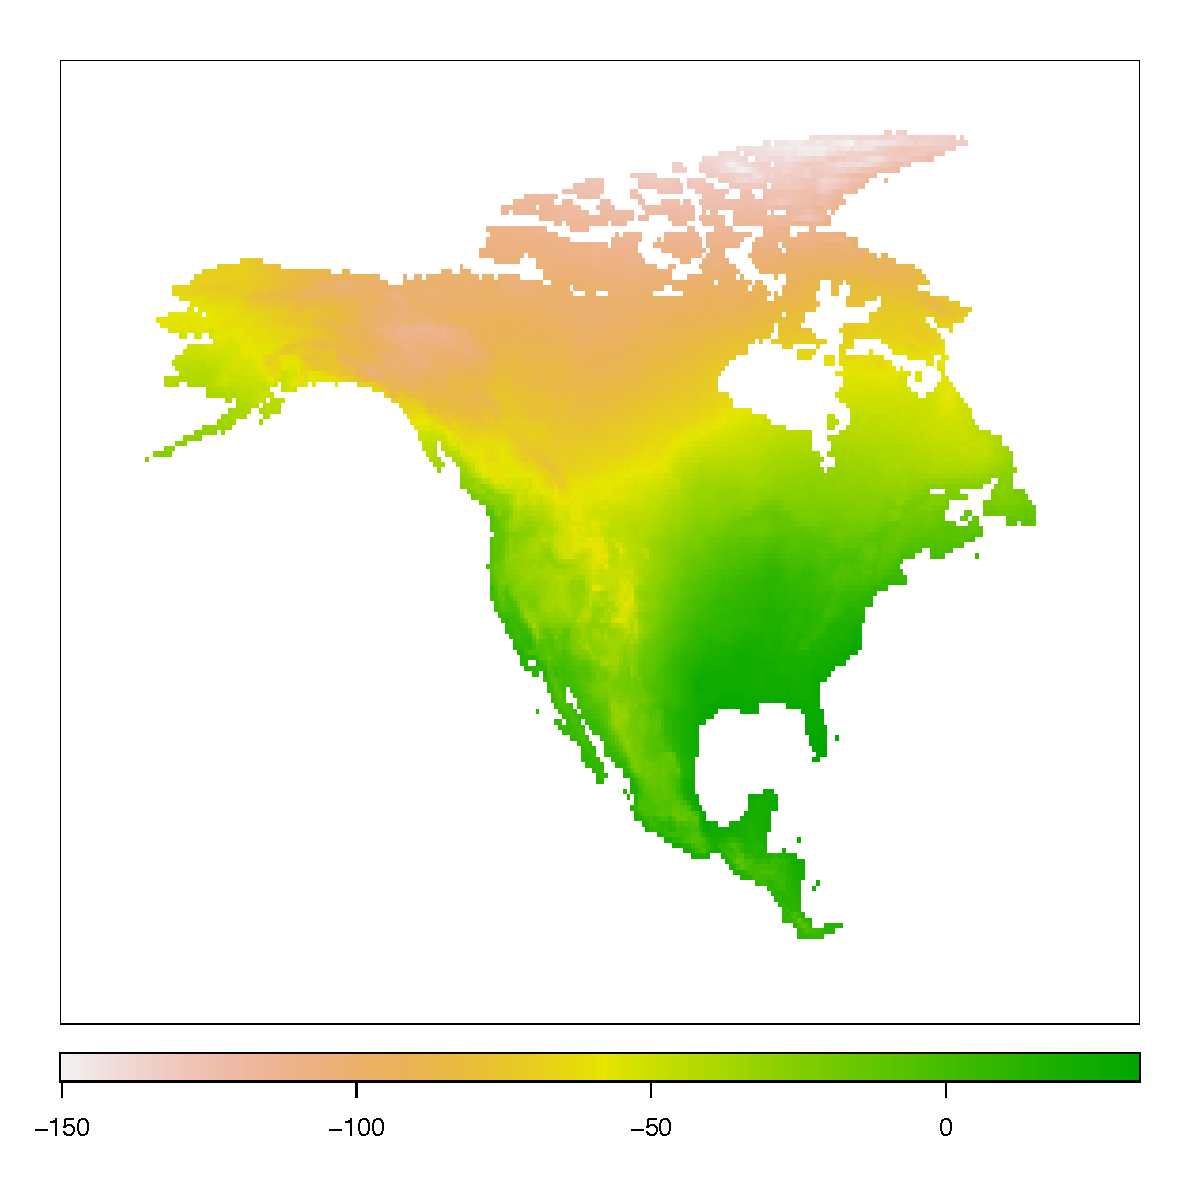
\includegraphics[width=0.5\textwidth]{figs/isoscape.pdf}
% \end{center}
% 
% \vfill
% 
% \end{frame}

%==================================================================================================

\begin{frame}
\frametitle{Combined Model}

\vfill

\begin{center}

Genetic \qquad\qquad\qquad\quad
Isotopic \qquad\qquad\qquad\quad
Combined

\end{center}

\begin{center}
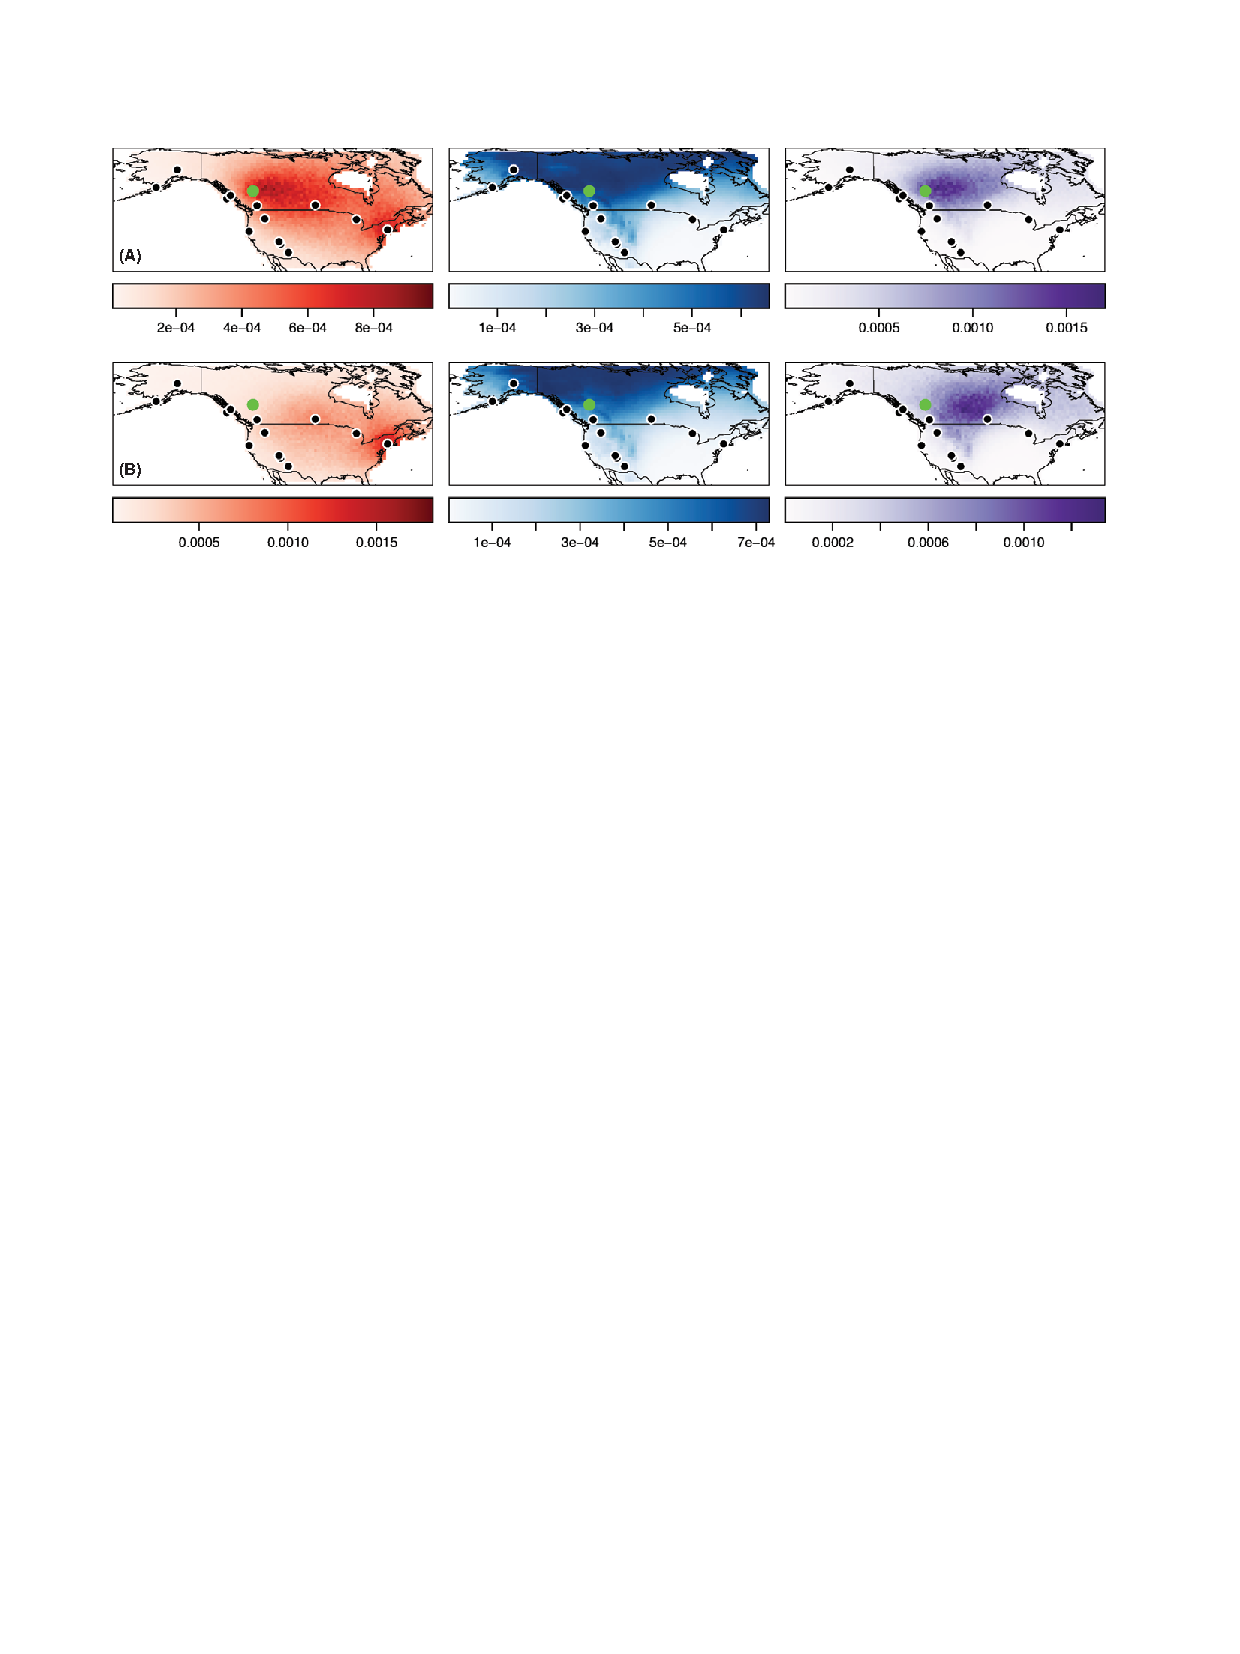
\includegraphics[width=\textwidth]{figs/hermit_maps.pdf}
\end{center}

\vfill

\end{frame}

%==================================================================================================

%\begin{frame}
%\frametitle{Model Assessment}
%
%\vspace{-3mm}
%
%\begin{center}
%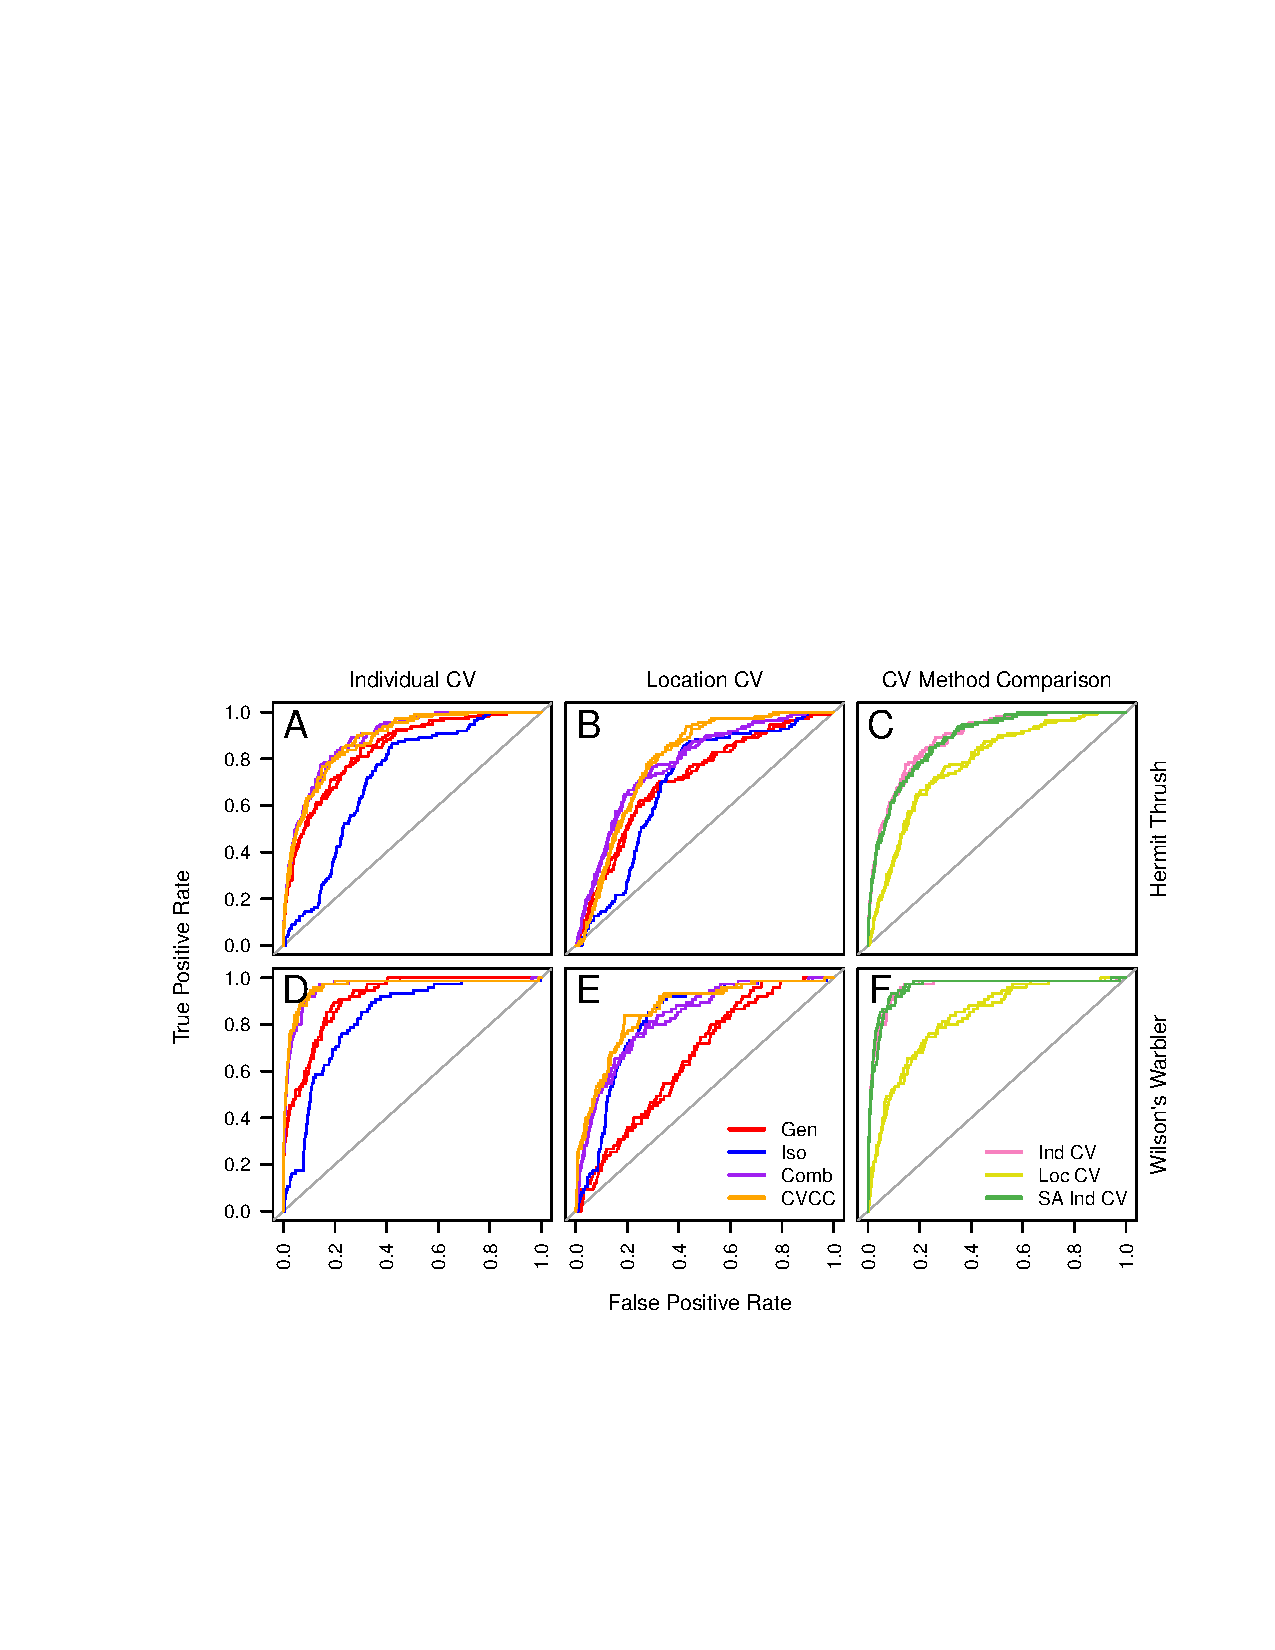
\includegraphics[width=\textwidth]{figs/ROCs.pdf}
%\end{center}
%
%\end{frame}

%==================================================================================================

\begin{frame}
\frametitle{Migratory Connectivity}

\vspace{-3mm}

\begin{center}
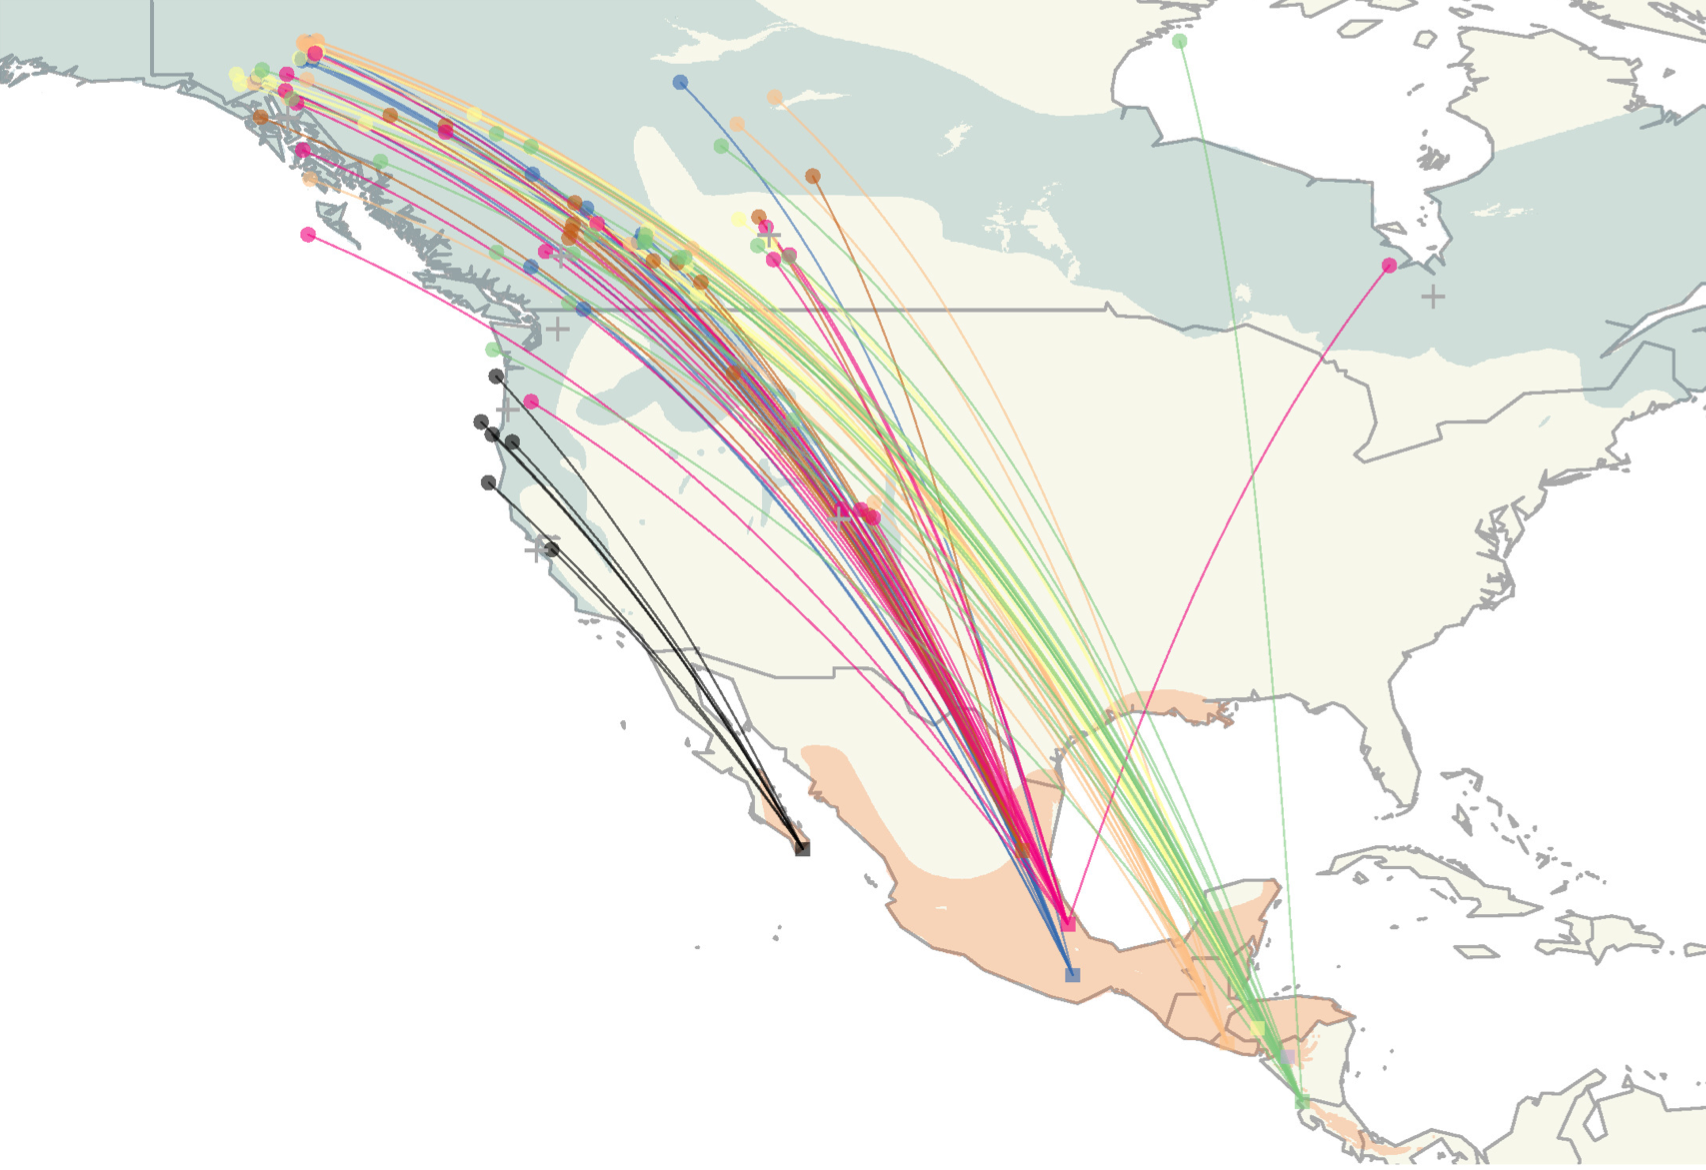
\includegraphics[width=0.9\textwidth]{figs/wintering.png}
\end{center}

\end{frame}

%==================================================================================================

\begin{frame}
\frametitle{Implementation}

Model fitting is done via MCMC (MH within Gibbs) \\
\begin{itemize} \addtolength{\itemsep}{3mm}
\item Original implementation in pure C++ with minimal dependencies (Wasser, et al. (2004))
\item Rewritten using R / C++ via Rcpp(Armadillo) 
\begin{itemize}
\item Code closer to matrix notation (and R)
\item Transparent use of high performance LAPACK implementations
\item R Package - isoscatR - \url{https://github.com/rundel/isoscatR}
\end{itemize}
\item Model fitting performance is quite good
\begin{itemize}
  \item 300,000 iterations in $\sim 5.5$ minutes
\end{itemize}
\item Bottleneck in drawing posterior predictive samples
\begin{itemize}
  \item1,000 iterations in $\sim 30$ minutes
\end{itemize}
\end{itemize}

\end{frame}

%==================================================================================================

\begin{frame}
\frametitle{Prediction details}

Why is the prediction slow? \pause 

\vspace{2mm}

Predicting allele frequencies for Hermit thrush at 3318 novel locations, in order to do this we sample from:
\[ \bm{\Theta}_p | \bm{\Theta}_m \sim \mathcal{N}(\bm{\mu}_p+\bm\Sigma_{pm}\bm\Sigma_{m}^{-1}(\bm{\Theta}_m-\bm\mu_m),\: \bm\Sigma_{p}-\bm\Sigma_{pm}\bm\Sigma_{m}^{-1}\bm\Sigma_{mp}) \]

\pause

\vspace{-3mm}

\begin{columns}
\column{0.10\textwidth}
\column{0.80\textwidth}
\begin{block}{Algorithm steps}
\begin{enumerate}
\item Calculate $\bm\Sigma_{pm}$, $\bm\Sigma_{p}$, and $\bm\Sigma_{p}-\bm\Sigma_{pm}\bm\Sigma_{m}^{-1}\bm\Sigma_{mp}$
\item Calculate $\text{Chol}(\bm\Sigma_{p}-\bm\Sigma_{pm}\bm\Sigma_{m}^{-1}\bm\Sigma_{mp})$
\item Sample from MVN
\item Calculate allele frequencies
\end{enumerate}
\end{block}
\column{0.1\textwidth}
\end{columns}
\end{frame}

%==================================================================================================

\begin{frame}
\frametitle{Posterior predictive sampling timings}

% Performance (CPU) :
% =============================================
% Step 1: 1.08 (0.0106)
% Step 2: 0.000174 (5.15e-06)
% Step 3: 0.467 (0.00171)
% Step 4: 0.0491 (0.000725)
% Step 5: 0.129 (0.000273)
% Step 6: 0.00654 (0.0338)


% Performance (CPU+GPU) :
% =============================================
% Step 1: 0.0462 (0.000196)
% Step 2: 3.43e-05 (3.02e-06)
% Step 3: 0.208 (0.000229)
% Step 4: 0.0525 (0.000227)
% Step 5: 0.127 (0.00188)
% Step 6: 0.032 (0.231)

\vspace{-7mm}

\begin{center}
\renewcommand*{\arraystretch}{1.5}
\begin{tabular}{rl|c|c|c}
& Step                                    & CPU (secs)  & CPU+GPU (secs)  & Rel. Performance \\
\hline
1. & Covariances                          & 1.080       & 0.046           & 23.0 \\
2. & Cholesky                             & 0.467       & 0.208           & 2.3 \\
3. & Sample                               & 0.049       & 0.052           & 0.9 \\
4. & Allele Freq                          & 0.129       & 0.127           & 1.0 \\
\hline 
   & Total                                & 1.732       & 0.465           & 3.7 \\
\end{tabular}

\end{center}

\vspace{3mm}
\only<2->{
\begin{columns}[t]

\column{0.42\textwidth}
Total run time: \\ \vspace{2mm}
\begin{itemize}
\item CPU - 28.9 mins
\item CPU+GPU - 7.8 mins
\end{itemize}

\column{0.58\textwidth}
\only<3>{
~\\ \vspace{5mm}
$\times \text{ CV runs} \; \left[\begin{array}{l}
166 \text{ for Hermit Thrush} \\
179 \text{ for Wilson's Warbler}
\end{array}\right]$
}
\end{columns}
}
\end{frame}

%==================================================================================================

\begin{frame}
\frametitle{Lessons}

Relatively small changes in one function resulted in 3 - 4x improvement

\begin{itemize}
\vspace{2mm} \item Cross validation results in two days instead of a week

\vspace{2mm} \item 1-2 weeks of implementation, 1 week of tweaking / testing

\vspace{2mm} \item Started with Cholesky, other optimizations followed
\end{itemize}

\vspace{7mm} \pause

Issues:

\begin{itemize}
\vspace{2mm} \item External library dependency makes package development \\ (much) more complicated

\vspace{2mm} \item Additional code verbosity and complexity

\end{itemize}

\end{frame}

%==================================================================================================

\begin{frame}
\frametitle{Improving Covariance Calculations}
    
Covariance is assumed to be stationary and isotropic
\begin{itemize}
\item Elements of the covariance matrix can be calculated independently
\item Small scale ``embarrassingly parallel''
\item Implementation is straight forward \\ (if we don't worry about things like symmetry)
\end{itemize}

\vfill
\begin{center}
\fbox{
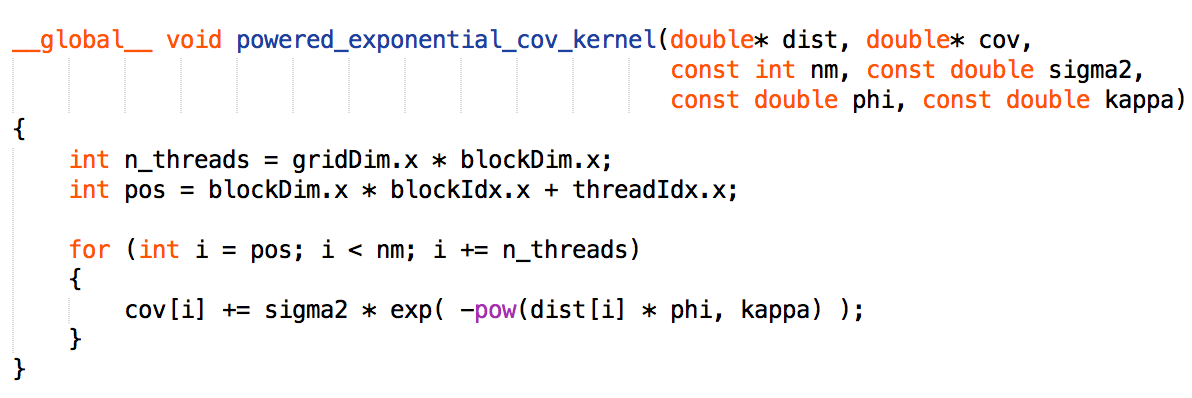
\includegraphics[width=0.95\textwidth]{figs/pow_exp_kernel.png}
}
\end{center}
\vfill

\end{frame}




%==================================================================================================

\begin{frame}
\frametitle{Building core tools}

Common set of (expensive) tasks for GP models

\vspace{1mm}

\begin{itemize}
\item Covariance calculation
\item Cholesky of Cov. 
\item Inverse of Cov. 
\end{itemize}

\vspace{2mm}

Goal is to make performing these tasks on a GPU as painless as possible and allow interoperability with GPU (magma, CUBLAS) and CPU (Armadillo) libraries.

\begin{itemize}
\item GPU matrix class
\item Modern resource management (RAII, move semantics)
\item Simple translation between GPU and CPU memory
\end{itemize}

\vfill

R Package - RcppGP - {\small \url{https://github.com/rundel/RcppGP}}

\end{frame}

%==================================================================================================

\begin{frame}[label=code]
\frametitle{CPU vs GPU code}

\vfill

\begin{center}
\fbox{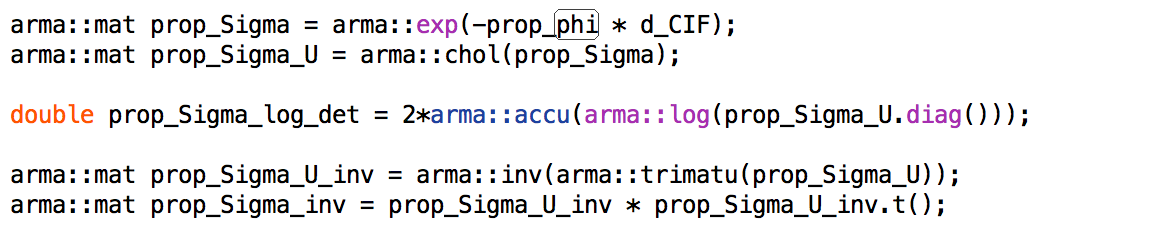
\includegraphics[width=0.9\textwidth]{figs/CPU.png}}

\vspace{10mm}

\fbox{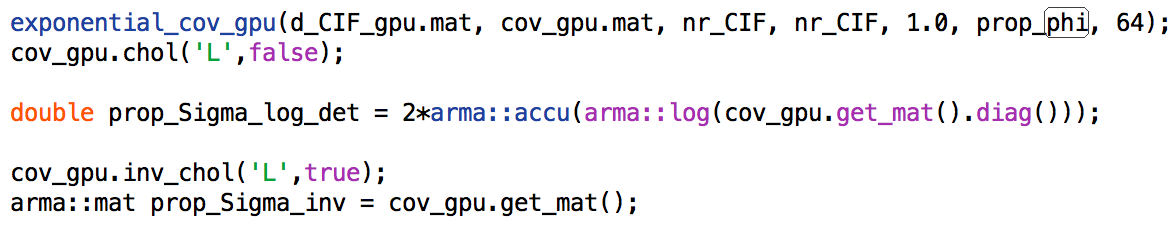
\includegraphics[width=0.9\textwidth]{figs/GPU.png}}
\end{center}

\vfill


\hyperlink{pm_lessons}{\beamerbutton{Back}}
\end{frame}


%==================================================================================================

\section{Speciated PM$_{2.5}$ Modeling}

%==================================================================================================

\begin{frame}
\frametitle{Background}
    
Fine particulate matter (\PM{}) is an EPA regulated air pollutant linked to a variety of adverse health effects

\begin{itemize}
  \vspace{2mm} \item Classified based on particle size ($<2.5$ $\mu$m diameter)
  \vspace{2mm} \item Major species: Sulfate, Nitrate, Ammonium, Soil, Carbon.
  \vspace{2mm} \item Minor species: trace elements (K, Mg, Ca), heavy metals (Cu, Fe), etc.
  \vspace{2mm} \item Complex spatio-temporal dependence between species
\end{itemize}


\end{frame}

%==================================================================================================

\begin{frame}
\frametitle{Data}

Speciated \PM Sources
\begin{itemize}
  \item Chemical Speciation Network (CSN) - 221 stations
  \item Interagency Monitoring of Protected Visual Environments (IMPROVE) - 172 stations
\end{itemize}

\vspace{1mm}

Total \PM Sources
\begin{itemize}
  \item Federal Reference Method (FRM) - 949 stations
\end{itemize}

\vspace{1mm}

Model Output
\begin{itemize}
  \item Community Multi-scale Air Quality (CMAQ) - 12 km grid
\end{itemize}

\vspace{1mm}

Data Issues
\begin{itemize}
  \item Monitoring frequency
  \item Total vs Sum of Species
\end{itemize}

\end{frame}


%==================================================================================================

\begin{frame}
\frametitle{Species Model Details}

For the 5 major species (Sulfate, Nitrate, Ammonium, Soil, Carbon) and the two networks (CSN, IMPROVE):
%
\begin{align*}
C_t^i(\bm{s}) &= Z_t^i(\bm{s}) + \epsilon_{C,t}^i(\bm{s}) \\
I_t^i(\bm{s}) &= Z_t^i(\bm{s}) + \epsilon_{I,t}^i(\bm{s})
\end{align*}

where $Z_t^i(\bm{s})$ are the latent ``true'' concentrations of species $i$ at time $t$ and locations $\bm{s}$, and is given by
%
\begin{align*}
{Z}_t^i(\bm{s}) &= \max{}\left(0,~\widetilde{Z}_t^i(\bm{s})\right) \\
\widetilde{Z}_t^i(\bm{s}) &= \beta_{0,t}^i +\beta_{0,t}^i(\bm{s}) + \beta_{1,t}^i \: Q_t^i(B_{\bm{s}})  
\end{align*}


\end{frame}

%==================================================================================================

\begin{frame}
\frametitle{Total \PM Model Details}

For total \PM from the three networks (CSN, IMPROVE, FRM):
%
\begin{align*}
C_t^{tot}(\bm{s}) &= Z_t^{tot}(\bm{s}) + \epsilon_{C,t}^{tot}(\bm{s}) \\
I_t^{tot}(\bm{s}) &= Z_t^{tot}(\bm{s}) + \epsilon_{I,t}^{tot}(\bm{s}) \\
F_t^{tot}(\bm{s}) &= Z_t^{tot}(\bm{s}) + \epsilon_{F,t}^{tot}(\bm{s})
\end{align*}

where $Z_t^{tot}(\bm{s})$ are the latent ``true'' concentration of total \PM at time $t$ and locations $\bm{s}$, which is given by the sum of the major species and the ``other'' species concentrations.
%
\[ Z^{tot}_{t}(\bm{s}) = \sum_{i=1}^{5} Z^i_t(\bm{s}) + Z^{o}_{t}(\bm{s}) \]

{\footnotesize
\[
{Z}_t^o(s) = \max{}\left(0,~\widetilde{Z}_t^o(s)\right) \qquad
\widetilde{Z}_t^{o}(\bm{s}) = \beta_{0,t}^o +\beta_{0,t}^o(\bm{s}) + \beta_{1,t}^o \: Q_t^o(B_{\bm{s}})
\]
}

\end{frame}

%==================================================================================================

\begin{frame}
\frametitle{Spatial Dependence}

Spatial dependence enters the model through the $\beta_{0,t}^i(s)$ parameters for $i \in \{o,1,2,3,4,5\}$.
%
\vspace{1mm}
\[ \beta_{0,t}^i(\bm{s}) = {\sigma}^i_t~w^i_t(\bm{s}) \]
%

where $w^i_{t}(\bm{s})$ are zero mean, variance $1$, Gaussian processes with exponential correlation given by 
%
\vspace{1mm}
\begin{align*}
\text{corr}(w^i_{t}(\bm{s}),w^i_{t}(\bm{s}')) = \exp(-\phi^i_{t} |\bm{s}-\bm{s}'|)
\end{align*}

Additional dependence between species is introduces via coregionalization,

\[
 \left( \begin{array}{cc} \beta^i_{0,t}(\boldsymbol{s})\\ \beta^j_{0,t}(\boldsymbol{s}) \end{array} \right)
 = \boldsymbol{A}_t \left( \begin{array}{cc} w^i_t(\boldsymbol{s})\\ w^j_t(\boldsymbol{s}) \end{array} \right).
\]

\end{frame}

%==================================================================================================

% \begin{frame}
% \frametitle{Model Details}

% For each species and network,

% \vspace{-5mm}

% \begin{columns}[t]
% \column{0.4\textwidth}
% \begin{align*}
% C_t^i(\bm{s}) &= Z_t^i(\bm{s}) + \epsilon_{C,t}^i(\bm{s}) \\
% I_t^i(\bm{s}) &= Z_t^i(\bm{s}) + \epsilon_{I,t}^i(\bm{s}) \\
% \end{align*}

% \column{0.6\textwidth}\pause
% \begin{align*}
% {Z}_t^i(\bm{s}) &= \max{}\left(0,~\widetilde{Z}_t^i(\bm{s})\right) \\
% \widetilde{Z}_t^i(\bm{s}) &= \beta_{0,t}^i +\beta_{0,t}^i(\bm{s}) + \beta_{1,t}^i \: Q_t^i(B_{\bm{s}})  
% \end{align*}
% \end{columns}

% \vspace{2mm} \pause

% For total PM,
% \begin{columns}[c]
% \column{0.42\textwidth}
% \begin{align*}
% C_t^{tot}(\bm{s}) &= Z_t^{tot}(\bm{s}) + \epsilon_{C,t}^{tot}(\bm{s}) \\
% I_t^{tot}(\bm{s}) &= Z_t^{tot}(\bm{s}) + \epsilon_{I,t}^{tot}(\bm{s}) \\
% F_t^{tot}(\bm{s}) &= Z_t^{tot}(\bm{s}) + \epsilon_{F,t}^{tot}(\bm{s})
% \end{align*}

% \column{0.58\textwidth} \pause
% \vspace{6mm}
% \[ Z^{tot}_{t}(\bm{s}) = \sum_{i=1}^{5} Z^i_t(\bm{s}) + Z^{o}_{t}(\bm{s}) \]
% \end{columns}

% \vspace{3mm} \pause

% \begin{align*}
% {Z}_t^o(s) &= \max{}\left(0,~\widetilde{Z}_t^o(s)\right) \\
% \widetilde{Z}_t^{o}(\bm{s}) &= \beta_{0,t}^o +\beta_{0,t}^o(\bm{s}) + \beta_{1,t}^o \: Q_t^o(B_{\bm{s}})
% \end{align*}

% \end{frame}

% %==================================================================================================

% \begin{frame}
% \frametitle{Model Details Cont.}

% Spatial dependence enters the model through the $\beta_{0,t}^i(s)$ and $\beta_{0,t}^o(s)$ parameters.


% \[ \beta_{0,t}^i(\bm{s}) = {\sigma}^i_t~w^i_t(\bm{s}) 
% \hspace{10mm}
% \beta_{0,t}^o(\bm{s}) = {\sigma}^o_t~w^o_t(\bm{s}) \]

% \vspace{5mm}

% where $w^i_{t}(\bm{s})$ and $w^o_{t}(\bm{s})$ are zero mean, variance $1$, Gaussian processes with exponential correlation given by 


% \begin{align*}
% \text{corr}(w^i_{t}(\bm{s}),w^i_{t}(\bm{s}')) = \exp(-\phi^i_{t} |\bm{s}-\bm{s}'|) \\
% \\
% \text{corr}(w^o_{t}(\bm{s}),w^o_{t}(\bm{s}')) = \exp(-\phi^o_{t} |\bm{s}-\bm{s}'|)
% \end{align*}


% \end{frame}

%==================================================================================================

\begin{frame}[label=pm_results]
\frametitle{Model results}

\vfill

\begin{center}
\only<1>{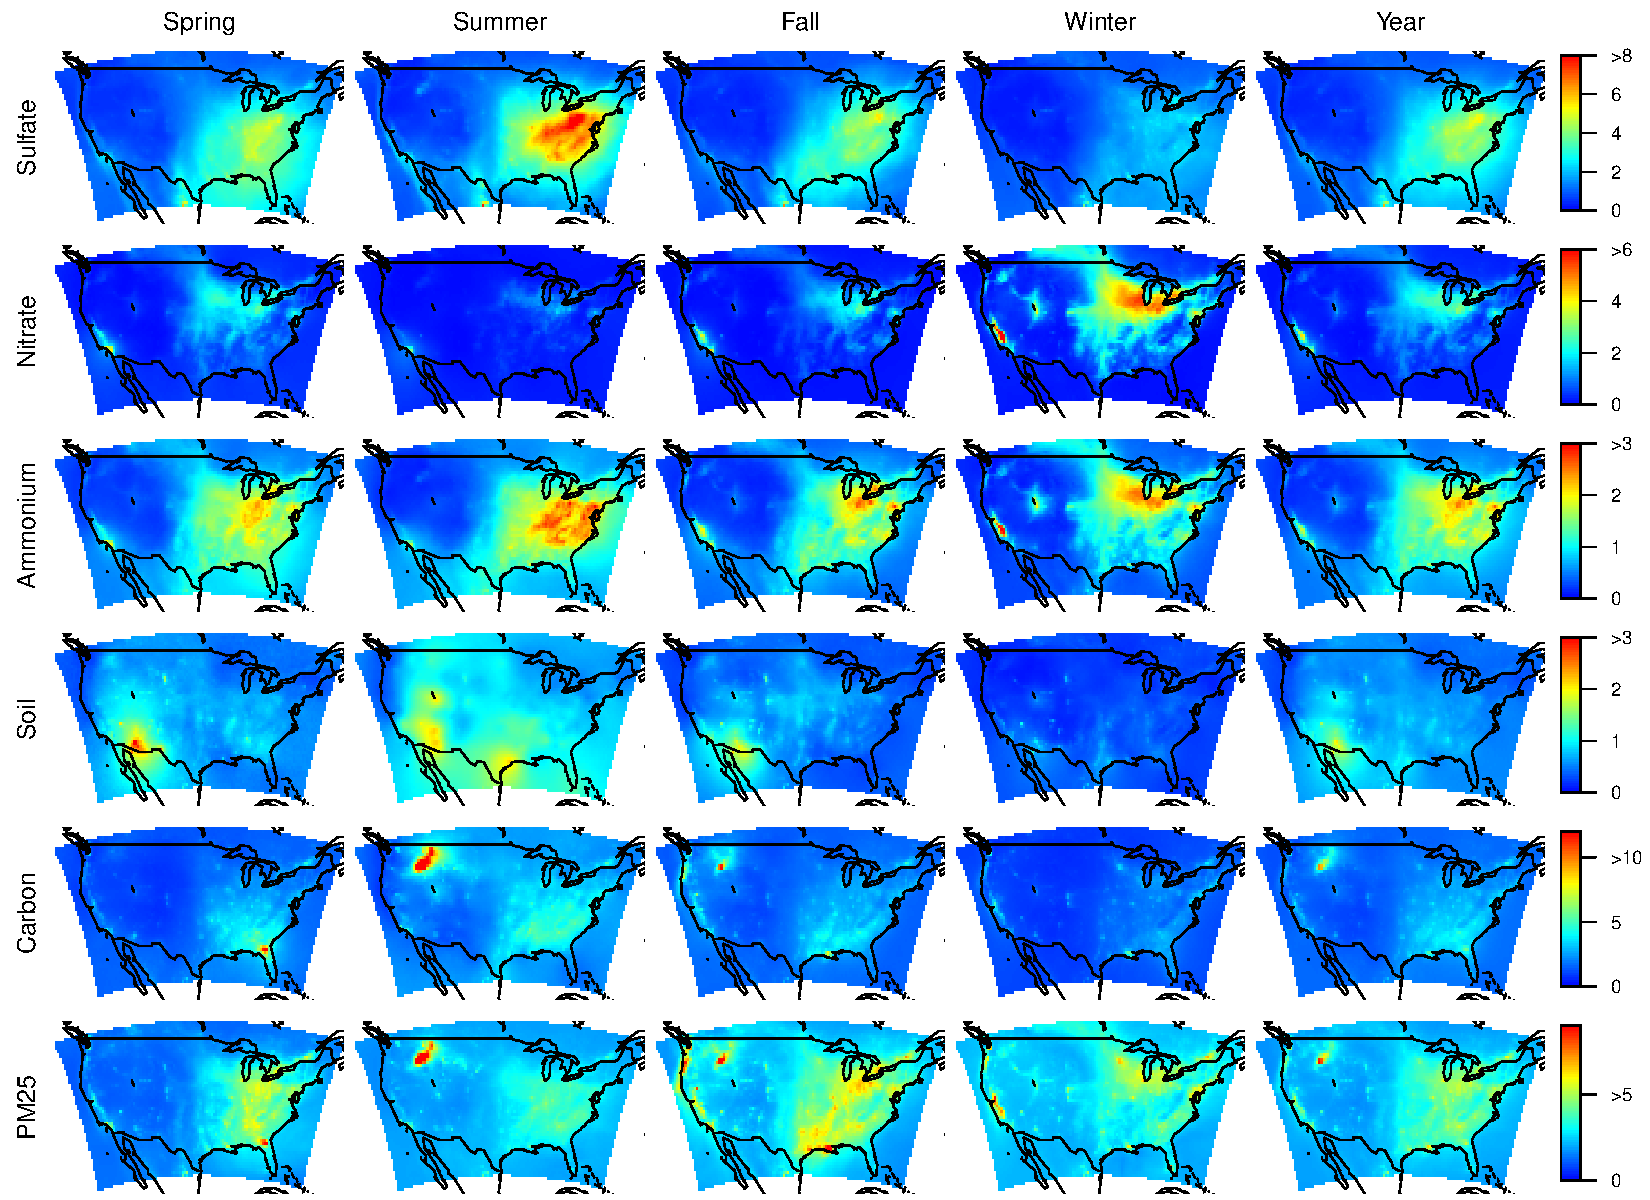
\includegraphics[width=0.8\textwidth]{figs/pm_maps.pdf}}
\only<2>{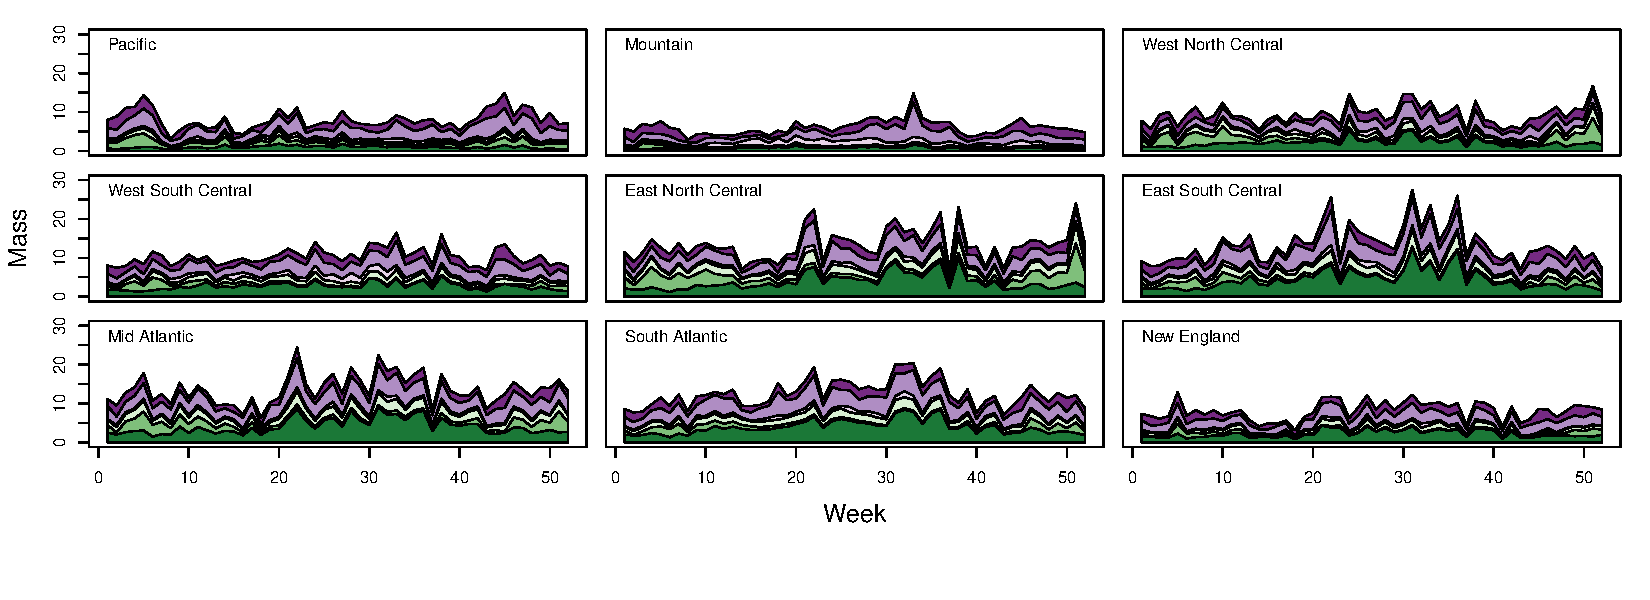
\includegraphics[width=\textwidth]{figs/pm_ts.pdf}\\
         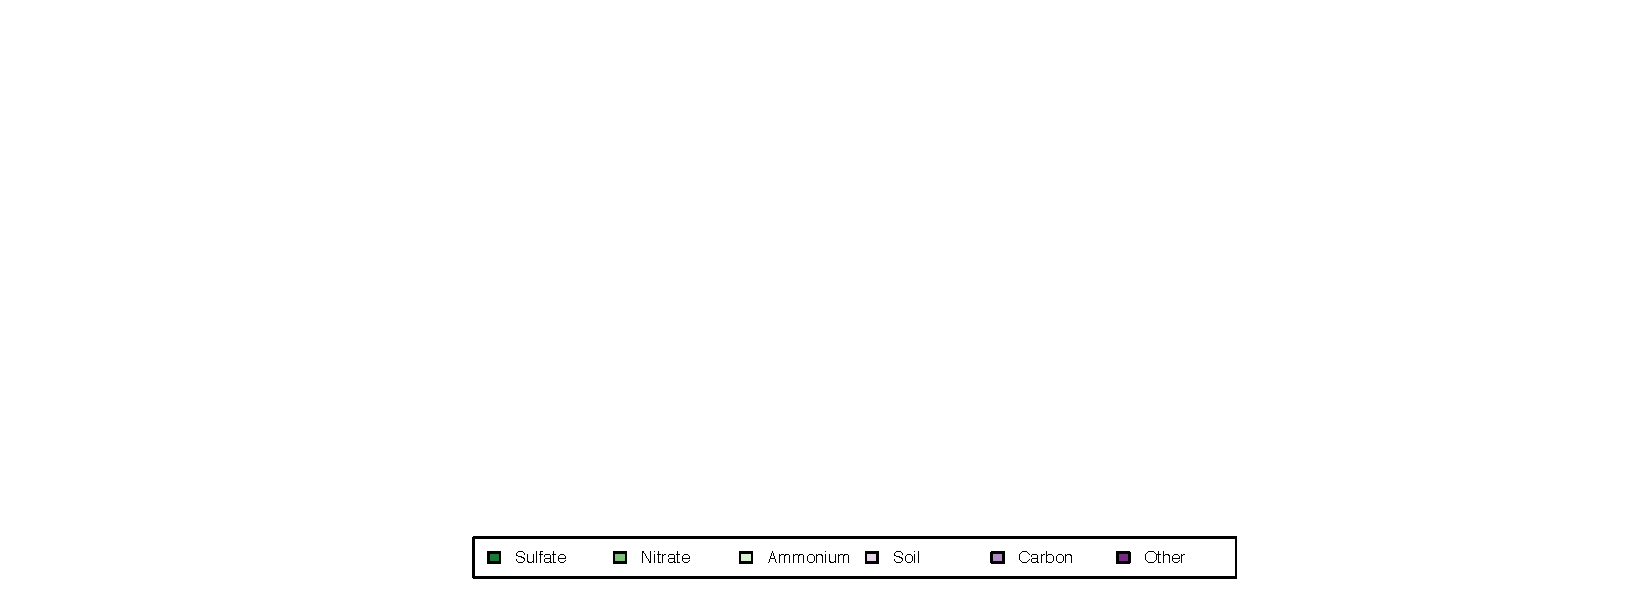
\includegraphics[width=0.7\textwidth]{figs/pm_ts_legend.pdf}}
\end{center}

\vfill

\end{frame}

%==================================================================================================

\begin{frame}
\frametitle{MCMC performance}

\begin{center}
\renewcommand*{\arraystretch}{1.5}
\begin{tabular}{l|c|c|c}
Parameter                 & CPU (secs) & CPU+GPU (secs)  & Rel. Performance \\
\hline
$\beta_0, \; \beta_1$     & 0.00029    & 0.00030         & 0.97 \\
$\beta_0(s) $             & 0.09205    & 0.09132         & 1.00 \\
$\sigma^2$                & 0.00383    & 0.00385         & 0.99 \\
$\phi$                    & 0.46084    & 0.25174         & 1.83 \\
$\tau^2_i,\; \tau^2_{tot}$& 0.00003    & 0.00003         & 1.00 \\
\hline
Total                     & 0.55708    & 0.34729         & 1.60
\end{tabular}
\end{center}

\end{frame}

%==================================================================================================

\begin{frame}
\frametitle{Run times}

Total run time for model fitting (50,000 iterations): \\ \vspace{2mm}

\begin{columns}[c]
\column{0.5\textwidth}
\begin{itemize}
\item CPU - 7.7 hours
\item CPU+GPU - 4.8 hours
\end{itemize}
\column{0.5\textwidth}
$\times$ 52 weeks
\end{columns}

\vspace{2mm} \pause

Total run time for model prediction at 5950 locations (1,000 iterations): \\ \vspace{2mm}

\begin{columns}[c]
\column{0.5\textwidth}
\begin{itemize}
\item CPU - 7.2 hours
\item CPU+GPU - 4.3 hours
\end{itemize}
\column{0.5\textwidth}
$\times$ 52 weeks
\end{columns}

\vspace{2mm}\pause

One run takes about 775 hours (4.6 days) total on CPU alone, 473 (2.8 days) on CPU and GPU. 

\pause

\begin{center}
$\times$ 3 model variants\\
$\times$ 10 for cross validation
\end{center}

\end{frame}

%==================================================================================================

\begin{frame}[label=pm_lessons]
\frametitle{Lessons}

Established infrastructure makes a huge difference in development time
\begin{itemize}
  \item 1 hour to go from CPU implementation to CPU+GPU implementation 
  \item Code shown previously is 2/3 of the changes necessary \hyperlink{code}{\beamerbutton{Code}}
\end{itemize}

\vspace{2mm}
In practice, was easier to run CPU only code across more servers (configuration time / effort)

\begin{itemize}
\item Not possible (or at least easy) for models variants that are not independent in time.
\item There are $\sim20$ desktops with GPUs available in the department (available via Condor)
\end{itemize}

\end{frame}

%==================================================================================================

\section{GPUs and Low Rank Approximations}

%==================================================================================================

\begin{frame}
\frametitle{Low rank approximations}

For a Gaussian process

\[ Y(\bm{s}) = x(\bm{s})' \, \bm{\beta} + w(\bm{s}) + \epsilon, \quad \epsilon \sim N(0,~\tau^2 \, I) \]
%
\[ w(\bm{s}) \sim N(0,~\bm{C}(\bm{s})), \quad \bm{C}(\bm{s},\bm{s}')=\sigma\,\rho(\bm{s},\bm{s}'|\theta) \]

if we can approximate $\bm{C}(\bm{s})$ with a low rank approximation with the form $\bm{U}\,\bm{S}\,\bm{V}'$ where $\bm{U}$ and $\bm{V}$ are $n \times k$ and $\bm{S}$ is $k \times k$.

~\\\pause

We can the use of the Sherman-Morrison-Woodbury formula for the inverse (and determinant),

\[
\bm{C}(\bm{s})^{-1} \approx
\left(\bm{A} + \bm{U}\bm{S}\bm{V'}\right)^{-1} = 
\bm{A}^{-1} - \bm{A}^{-1} \bm{U} \left(\bm{S}^{-1}+\bm{V}' \bm{A}^{-1} \bm{U}\right)^{-1}\bm{V}' \bm{A}^{-1}.
\]


\end{frame}

%==================================================================================================

\begin{frame}
\frametitle{Gaussian Predictive Processes}

For a rank $k$ approximation,

\begin{itemize}
\item Pick $k$ knot locations $\bm{s}^*$
\item Calculate knot covariance ($\bm{C}(\bm{s}^*)$) and knot cross-covariance ($\bm{C}(\bm{s}^*)^{-1}$)
\item Approximate full covariance
\end{itemize}
%
\[\bm{C}(\bm{s}) \approx \bm{C}(\bm{s},\bm{s}^*) \, \bm{C}(\bm{s}^*)^{-1} \, \bm{C}(\bm{s}^*,\bm{s}).\]


\begin{itemize}
\item Systematically underestimates variance, inflates $\tau^2$. 

\item Modified predictive process corrects this using 
%
\vspace{1mm}
{\small
\[
\bm{C}(\bm{s}) \approx
\bm{C}(\bm{s},\bm{s}^*) \, \bm{C}(\bm{s}^*)^{-1} \, \bm{C}(\bm{s}^*,\bm{s}) + \text{diag}\Big(\bm{C}(\bm{s}) - \bm{C}(\bm{s},\bm{s}^*) \, \bm{C}(\bm{s}^*)^{-1} \, \bm{C}(\bm{s}^*,\bm{s})\Big).
\]
}
\end{itemize}

\vvfill

{\footnotesize
\begin{center}
Banerjee, Gelfand, Finley, Sang (2008), Finley, Sang, Banerjee, Gelfand (2008)
\end{center}
}
\end{frame}

%==================================================================================================

\begin{frame}
\frametitle{Low Rank Approximations via Random Projections}

\begin{enumerate}
\item Starting with an $m \times n$ matrix $\bm{A}$.
\item Draw an $n \times k+p$ Gaussian random matrix $\bm{\Omega}$.
\item Form $\bm{Y} = \bm{A}\,\bm{\Omega}$ and compute its QR factorization $\bm{Y} = \bm{Q}\,\bm{R}$
%\item For $j=1,2,\ldots,q$ where q is integer power
%   Form Y􏱷 = AT Q and compute its QR factorization Y􏱷 = Q􏱷 R􏱷 j j−1 j jj
%   Form Yj = AQ􏱷j and compute its QR factorization Yj = Qj Rj
%   End
%\item $Q = Q_q$
\item Form the $k+p \times n$ matrix $\bm{B}=\bm{Q}'\,\bm{A}$.
\item Compute the SVD of the small matrix $\bm{B}$, $\bm{B} = \bm{\hat{U}}\,\bm{S}\,\bm{V}'$.
\item Form the matrix $\bm{U} = \bm{Q} \, \bm{\hat{U}}$.
\end{enumerate}

~\\ \pause

Resulting approximation has nicely bounded expected error,
%
\vspace{1mm}
\[ \text{E } \, \| \bm{A} - \bm{U}\bm{S}\bm{V}'\| \leq \left[1 + \frac{4\sqrt{k+p}}{p-1} \sqrt{\min(m,n)} \right] \sigma_{k+1}. \]

\vvfill

{\footnotesize
\begin{center}
Halko, Martinsson, Tropp (2011)
\end{center}
}
\end{frame}


%==================================================================================================

\begin{frame}
\frametitle{Random Matrix Low Rank Decompositions and GPs}

Preceding algorithm can be modified slightly to take advantage of the positive definite structure of a covariance matrix.

\begin{enumerate}
\item Starting with an $n \times n$ covariance matrix $\bm{A}$.
\item Draw an $n \times k+p$ Gaussian random matrix $\bm{\Omega}$.
\item Form $\bm{Y} = \bm{A}\,\bm{\Omega}$ and compute its QR factorization $\bm{Y} = \bm{Q}\,\bm{R}$
\item Form the $k+p \times k+p$ matrix $\bm{B}=\bm{Q}'\,\bm{A} \, \bm{Q}$.
\item Compute the eigen decomposition of the small matrix $\bm{B}$, $\bm{B} = \bm{\hat{U}}\,\bm{S}\,\bm{\hat{U}}'$.
\item Form the matrix $\bm{U} = \bm{Q} \, \bm{\hat{U}}$.
\end{enumerate}

Once again we have a bound on the error,
%
\vspace{1mm}
\[
   \text{E } \| \bm{A} - \bm{Q}(\bm{Q}'\bm{A}\bm{Q})\bm{Q}'\| 
 = \text{E } \| \bm{A} - \bm{U}\bm{S}\bm{U}'\| 
\lessapprox c \cdot \sigma_{k+1}. 
\]

\vvfill

{\footnotesize
\begin{center}
Halko, Martinsson, Tropp (2011), Banerjee, Dunson, Tokdar (2012)
\end{center}
}

\end{frame}


%==================================================================================================

\begin{frame}[fragile]
\frametitle{Low Rank Approximations and GPUs}

Both predictive process and random matrix low rank approximations are good candidates for acceleration using GPUs.

\begin{itemize}
\item Both use Sherman-Woodbury-Morrison to calculate the inverse (involves matrix multiplication, addition, and a small Matrix inverse).

\item Predictive processes involves several covariance matrix calculations (knots and cross-covariance) and a small matrix inverse.

\item Random matrix low rank involves a large matrix multiplication ($\bm{A}\bm{\Omega}$) and several small matrix decompositions (QR, eigen).

\item Functionality for both approaches included in current version of RcppGP (inv\_lr and
inv\_pp).

\end{itemize}

\end{frame}

%==================================================================================================




\begin{frame}
\frametitle{Matrix inverse (fixed rank, strong dependence)}

\vspace{-8mm}

\only<1>{
\begin{center}
\begin{knitrout}\footnotesize
\definecolor{shadecolor}{rgb}{0.969, 0.969, 0.969}\color{fgcolor}

{\centering 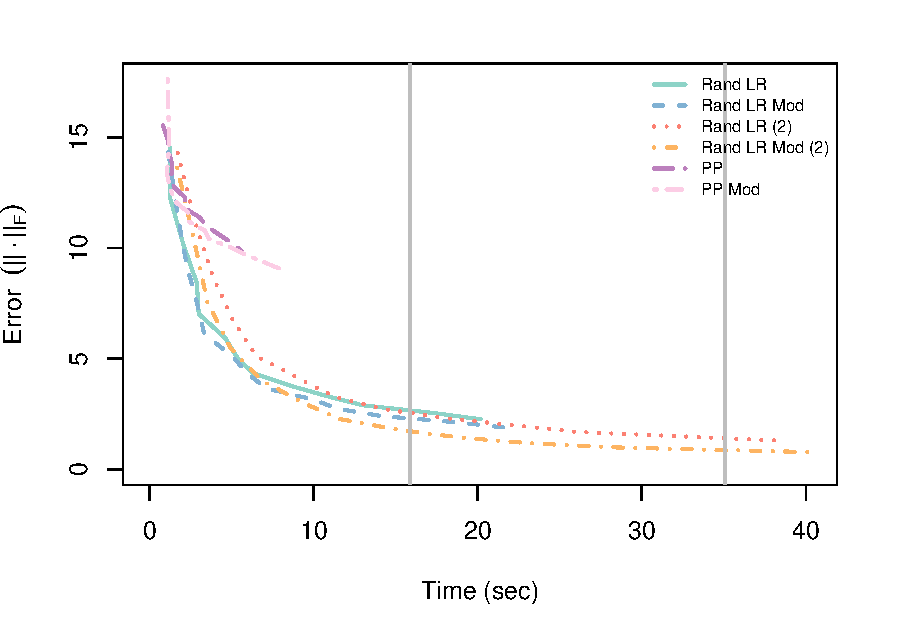
\includegraphics[width=0.95\textwidth]{plots/unnamed-chunk-3-1} 

}



\end{knitrout}
\end{center}
}

\only<2>{
\begin{center}
\begin{knitrout}\footnotesize
\definecolor{shadecolor}{rgb}{0.969, 0.969, 0.969}\color{fgcolor}

{\centering 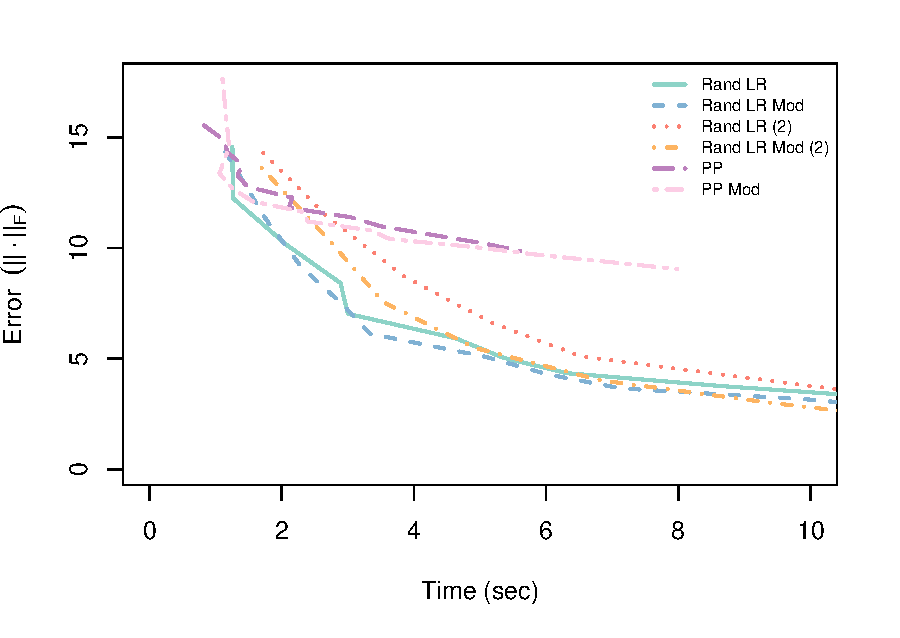
\includegraphics[width=0.95\textwidth]{plots/unnamed-chunk-4-1} 

}



\end{knitrout}
\end{center}
}

\vspace{-10mm}
\[ n = 15000,\quad k=\{100,\ldots,4900\} \]

\end{frame}

%==================================================================================================

\begin{frame}
\frametitle{Matrix inverse (fixed rank, weak dependence)}

\vspace{-8mm}

\only<1>{
\begin{center}
\begin{knitrout}\footnotesize
\definecolor{shadecolor}{rgb}{0.969, 0.969, 0.969}\color{fgcolor}

{\centering 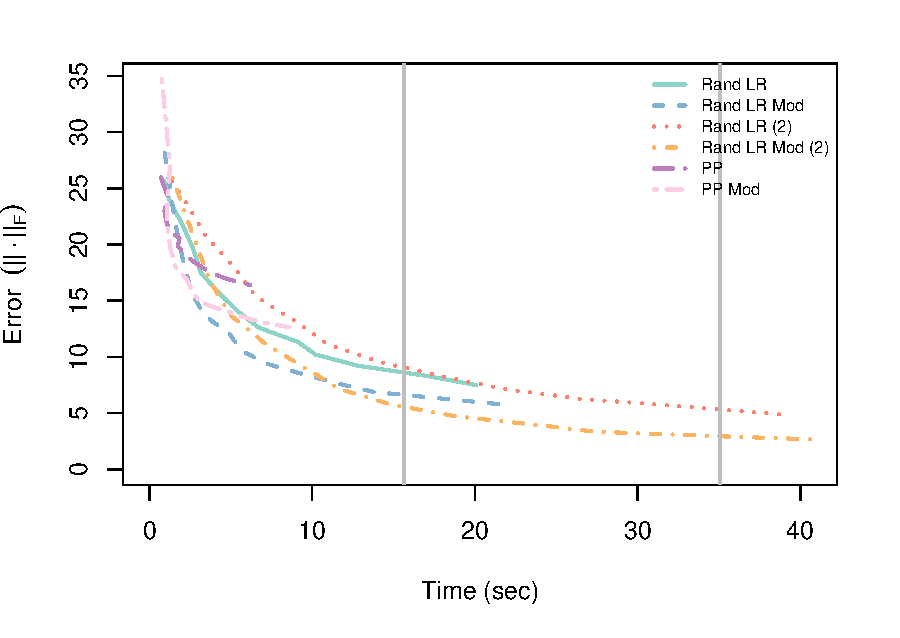
\includegraphics[width=0.95\textwidth]{plots/unnamed-chunk-5-1} 

}



\end{knitrout}
\end{center}
}

\only<2>{
\begin{center}
\begin{knitrout}\footnotesize
\definecolor{shadecolor}{rgb}{0.969, 0.969, 0.969}\color{fgcolor}

{\centering 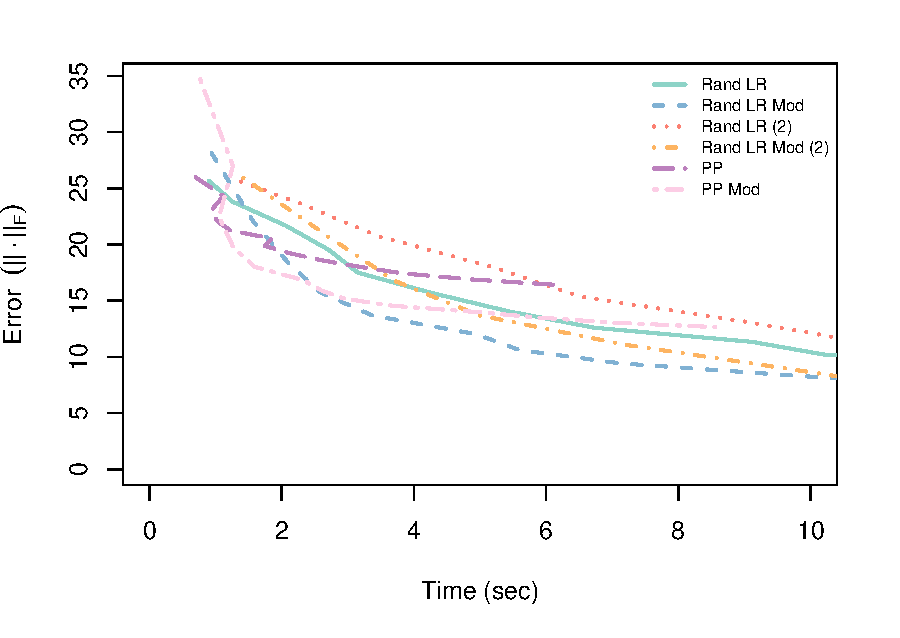
\includegraphics[width=0.95\textwidth]{plots/unnamed-chunk-6-1} 

}



\end{knitrout}
\end{center}
}

\vspace{-10mm}
\[ n = 15000,\quad k=\{100,\ldots,4900\} \]

\end{frame}


%==================================================================================================

\begin{frame}
\frametitle{Rand. Matrix Low Rank Decompositions for Prediction}

\vspace{-3mm}

This approach can also be used for prediction, if we want to sample 
\[ \mathcal{N}(0,\bm{\Sigma}) \text{ with }\Sigma \approx \bm{U} \bm{S} \bm{U}' = (\bm{U} \bm{S}^{1/2} \bm{U}')(\bm{U} \bm{S}^{1/2} \bm{U}')'\] 
then $X_{pred} = (\bm{U}\, \bm{S}^{1/2}\,\bm{U}') \times \bm{Z}$ where $Z_i \sim \mathcal{N}(0,1)$.

\pause

\begin{center}
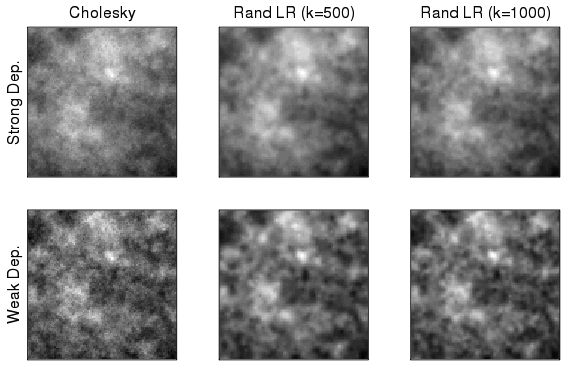
\includegraphics[width=0.6\textwidth]{figs/RandLRPred.png}
\end{center}

\vspace{-10mm}

\[ n=1000, \quad p=10000 \]

\begin{center}
{\footnotesize
Dehdari, Deutsch (2012)
}
\end{center}

\end{frame}

%==================================================================================================

\begin{frame}
\frametitle{Future Directions}

\begin{itemize}

\item Refinement of RcppGP

\vspace{1mm}
\begin{itemize}
  \vspace{1mm} \item Transition to header only implementation
  \vspace{1mm} \item Transparent GPU to CPU failover
  \vspace{1mm} \item Support for fixed error (instead of rank) random matrix low rank decomposition
  \vspace{1mm} \item Thinking about out-of-memory based approaches
\end{itemize}

\vspace{1mm}

\item Future of GPUs, CUDA, and Magma

\vspace{1mm}

\begin{itemize}
  \vspace{1mm} \item Single vs. Multi-GPU algorithms
  \vspace{1mm} \item Mixed precision algorithms
  \vspace{1mm} \item NVBLAS
  \vspace{1mm} \item Unified memory
  \vspace{1mm} \item cuSolver
\end{itemize}

\end{itemize}

\end{frame}


%==================================================================================================

\begin{frame}
\frametitle{Acknowledgments}

\begin{columns}[t]
\column{0.5\textwidth}
\textbf{Migratory Connectivity}
\vspace{5mm}
\begin{itemize}
  \item John Novembre - UChicago
  \item Thomas Smith - UCLA
  \item Kristen Ruegg - UCLA, UCSC
  \item Center for Tropical Research, UCLA IoES
\end{itemize}

\column{0.5\textwidth}
\textbf{Speciated \PM}
\vspace{2.5mm}
\begin{itemize}
  \item Alan Gelfand - Duke
  \item Dave Holland - EPA
  \item Erin Schliep - Missouri
\end{itemize}
\end{columns}

\vfill

\begin{center}
\begin{tabular}{ll}
RcppGP & \url{https://github.com/rundel/RcppGP} \\ 
\end{tabular}
\end{center}

\end{frame}


\end{document}
